\documentclass{article}
\title{Notas de Aula - MAT01057}
\author{Leonardo Suarez}
\date{\today}
\usepackage{macros}

\begin{document}
\maketitle

Notas de aula de Análise Matemática A, disciplina ministrada pelo prof. Paulo Zingano no semestre 25/1.

\tableofcontents

\section{Conjuntos Finitos e Infinitos}

\subsection{Números naturais}

Caracteriza-se o conjunto \(\N\) dos números naturais da seguinte forma:

\begin{enumerate}
    \item[\textbf{AI}] Existe uma função injetiva \(s : \N \to \N\) chamada \emph{função sucessor}, tal que \(s(n)\) é o sucessor de \(n\).
    \item[\textbf{AII}] Existe um único número natural \(1 \in \N\) tal que \(1 \neq s(n)\) para todo \(n \in \N\).
    \item[\textbf{AIII}] Se um conjunto \(X \subset \N\) é tal que \(1 \in X\) e \(s(X) \subset X\) (ie, \(n \in X \implies s(n) \in X\)), então \(X = \N\). (\emph{princípio da indução}.)
\end{enumerate}

\begin{defn} [soma, produto em \(\N\)]
    No conjunto \(\N\), definimos duas operações fundamentais: a \emph{adição} que associa a cada par de números \((m,n)\) sua \emph{soma} \(m+n\), e a \emph{multiplicação}, faz corresponder ao par \((m,n)\) seu \emph{produto} \(m\cdot n\). Definimos então:
    \begin{align}
        m + 1 &\coloneq s(m), \\
        m + s(n) &\coloneq s(m + n) \\
        m \cdot 1 &\coloneq m, \\
        m \cdot s(n) &\coloneq m \cdot n + m.
    \end{align}
\end{defn}

\begin{prop} [propriedades da adição e da multiplicação em \(\N\)]
    Sejam \(m, n, p \in \N\). Então:
    \begin{itemize}
        \item[(i)] \((m+n)+p = m+(n+p), \quad m \cdot (n \cdot p) = (m \cdot n) \cdot p\) (associatividade);
        \item[(ii)] \(m + n = n + m, \quad m \cdot n = n \cdot m\) (comutatividade);
        \item[(iii)] \(m \cdot (n + p) = m \cdot n + m \cdot p\) (distributividade);
        \item[(iv)] \(n + m = p + m \implies n = p, \quad n \cdot m = p \cdot m \implies n = p\) (lei do corte).
    \end{itemize} 
\end{prop}

\begin{defn} [ordem em \(\N\)]
    Dados \(m, n \in \N\), escreve-se \(m < n\) quando existe \(p \in \N\) tal que \(n = m + p\). Se \(m < n\) ou \(m = n\), escreve-se \(m \leq n\).
\end{defn}

\begin{thm} [princípio da boa-ordenação]
    Todo subconjunto não vazio \(A \subseteq \N\) possui um menor elemento, isto é, um elemento \(n_0 \in A\) tal que \(n_0 \leq n\) para todo \(n \in A\).
\end{thm}

\begin{proof}
    Sejam \(A \subseteq \N\) não vazio e \(I_n = \{p \in \N: p \neq n\}\). Se \(1 \in A\), é claro que \(1\) é o menor elemento de \(A\). Se \(1 \notin A\), considere o conjunto \(X = \{n \in \N: I_n \subseteq \N - A\}\).
    Nota que \(I_1 = \{1\} \subseteq \N - A\), logo \(1 \in X\). Como \(A\) é não vazio, tem-se que \(X \neq \N\), o que implica que existe \(n \in X\) tal que \(n_0 = n+1 \notin X\). Então \(n_0 \in A\), que é o menor elemento de \(A\), pois não existe número natural entre \(n\) e \(n+1\).
\end{proof}

\subsection{Conjuntos finitos}

\begin{defn}
    Um conjunto \(X\) diz-se \emph{finito} quando é vazio ou existem \(n \in \N\) e uma bijeção \(f: I_n \to X\). A bijeção \(f\) chama-se uma \emph{contagem} dos elementos de \(X\) e o número \(n\) chama-se o \emph{número cardinal} do conjunto finito \(X\).
\end{defn}

\begin{lem} \label{lema:bijecao}
    Se existe uma bijeção \(f: X \to Y\), então, dados \(a \in X\) e \(b \in Y\), existe também uma bijeção \(g: X \to Y\) tal que \(g(a) = b\).
\end{lem}

\begin{thm}
    Se \(A \subsetneq I_n\), não existe bijeção \(f: A \to I_n\).
\end{thm}

\begin{proof}
    Supõe, por absurdo, que o resultado é falso. Tome o menor natural \(n_0 \in \N\) tal que exista \(f: A \to I_{n_0}\) bijetiva. Se \(n_0 \in A\), pelo lema \eqref{lema:bijecao}, existe \(g: A \to I_{n_0}\) bijetiva tal que \(g(n_0)=n_0\).
    Então, a restrição de \(g\) a \(A - \{n_0\}\) é uma bijeção sobre \(I_{n_0 -1}\), o que contradiz a minimalidade de \(n_0\). Se \(n_0 \notin A\), pela sobrejetivdade de \(f\), existe \(a \in A\) tal que \(f(a)=n_0\), e a restrição de \(f\) ao subconjunto próprio \(A - \{a\}\) é uma bijeção sobre \(I_{n_0 -1}\), o que também leva a uma contradição.
\end{proof}

\begin{cor}
    Se \(f: I_m \to X\) e \(g: I_n \to X\) são bijeções, então \(m = n\).
\end{cor}

\begin{cor}
    Seja \(X\) um conjunto finito. Uma aplicação \(f: X \to X\) é injetiva sse é sobrejetiva.
\end{cor}

\begin{cor}
    Não existe uma bijeção entre um conjunto finito e um de seus subconjuntos próprios.
\end{cor}

\begin{thm}
    Todo subconjunto de um conjunto finito é finito.
\end{thm}

\begin{cor}
    Dada \(f: X \to Y\), se \(Y\) é finito e \(f\) é injetiva, então \(X\) é finito; se \(X\) é finito e \(f\) é sobrejetiva, então \(Y\) é finito.
\end{cor}

\begin{defn}
    Um subconjunto \(X \subseteq \N\) diz-se \emph{limitado} quando existe \(p \in \N\) tal que \(x \leq p\) para todo \(x \in X\).
\end{defn}

\begin{cor}
    Um subconjunto \(X \subseteq \N\) é finito sse é limitado.
\end{cor}

\subsection{Conjuntos infinitos}

\begin{defn}
    Diz-se que um conjunto \(X\) é \emph{infinito} quando não é finito, isto é, quando não é vazio nem existe bijeção \(f: I_n \to X\) para qualquer \(n \in \N\).
\end{defn}

\begin{thm}
    Se \(X\) é infinito, então existe uma aplicação injetiva \(f: \N \to X\).
\end{thm}

\begin{cor}
    Um conjunto \(X\) é infinito sse existe uma bijeção \(\phi: X \to Y\) sobre um subconjunto próprio \(Y \subseteq X\).
\end{cor}

\subsection{Conjuntos enumeráveis}

\begin{defn}
    Um conjunto \(X\) diz-se \emph{enumerável} quando é finito ou quando existe bijeção \(f: \N \to X\). Neste caso, \(f\) chama-se uma \emph{enumeração} dos elementos de \(X\).
\end{defn}

\begin{thm}
    Todo subconjunto \(X \subseteq \N\) é enumerável.
\end{thm}

\begin{cor}
    Seja \(f: X \to Y\) injetiva. Se \(Y\) é enumerável, então \(X\) também é. Em particular, todo subconjunto de um conjunto enumerável é enumerável.
\end{cor}

\begin{cor}
    Seja \(f: X \to Y\) sobrejetiva. Se \(X\) é enumerável, então \(Y\) também é.
\end{cor}

\begin{cor}
    O produto cartesiano de dois conjuntos enumeráveis é enumerável.
\end{cor}

\begin{cor}
    A reunião de uma família de conjuntos enumeráveis é enumerável.
\end{cor}

\section{Números Reais}

\subsection{R é um corpo}

\begin{defn} [soma, produto em \(\R\)]
    Definimos duas operações binárias no conjunto \(\R\): a \emph{adição} que associa a cada par de números reais \((x,y)\) sua \emph{soma} \(x+y\), e a \emph{multiplicação}, que faz corresponder ao par \((x,y)\) seu \emph{produto} \(x \cdot y\).
\end{defn}

Essas operações satisfazem os seguintes axiomas.
\begin{enumerate}
    \item [\textbf{AI}] para quaisquer \(x, y, z \in \R\), tem-se \((x + y) + z = x + (y + z)\) e \((x \cdot y) \cdot z = x \cdot (y \cdot z)\). \hfill (associatividade)
    \item [\textbf{AII}] para quaisquer \(x, y \in \R\), tem-se \(x + y = y + x\) e \(x \cdot y = y \cdot x\). \hfill (comutatividade)
    \item [\textbf{AIII}] existem \(0, 1 \in \R\) distintos tais que, para todo \(x \in \R\), tem-se \(x + 0 = x\) e \(x \cdot 1 = x\). \hfill (elemento neutro)
    \item [\textbf{AIV}] para todo \(x \in \R\), existe \(-x \in \R\) tal que \(x + (-x) = 0\). Se \(x \neq 0\), então existe \(x^{-1} \in \R\) tal que \(x \cdot x^{-1} = 1\). \hfill (inverso)
    \item [\textbf{AV}] para quaisquer \(x, y, z \in \R\), tem-se \(x \cdot (y + z) = x \cdot y + x \cdot z\). \hfill (distributividade)
\end{enumerate}

\subsection{R é um corpo ordenado}

Existe um subconjunto \(\mathcal{P} \subset \R\), chamado de \emph{conjunto dos números positivos}, que satisfaz os seguintes axiomas.
\begin{enumerate}
    \item [\textbf{P1}] Se \(x, y \in \mathcal{P}\), então \(x + y \in \mathcal{P}\) e \(x \cdot y \in \mathcal{P}\).
    \item [\textbf{P2}] Para todo \(x \in \R\), exatamente uma das seguintes alternativas é verdadeira: \(x \in \mathcal{P}\), \(x = 0\) ou \(-x \in \mathcal{P}\).
\end{enumerate}

\begin{rem}
    Todo número real \(x \neq 0\) tem quadrado positivo. De fato, se \(x \in \mathcal{P}\) então \(x \cdot x = x^2 \in \mathcal{P}\) por P1. Se \(x \notin \mathcal{P}\) tem-se por P2 que \(-x \in \mathcal{P}\), logo \((-x) \cdot (-x) = x^2 \in \mathcal{P}\). Em particular, \(1\) é um número positivo, pois \(1 = 1^2\).
\end{rem}

\begin{defn}
    Escreve-se \(x<y\) e diz-se que \(x\) é \emph{menor do que} \(y\) quando \(y - x \in \mathcal{P}\), isto é, \(y = x+z\) para algum \(z \in \mathcal{P}\). Neste caso, escreve-se também \(y > x\) e diz-se que \(y\) é \emph{maior do que} \(x\). Em particular, \(x>0\) significa que \(x \in \mathcal{P}\) e \(x<0\) significa que \(-x \in \mathcal{P}\).
\end{defn}

\begin{prop} [propriedades da relação de ordem \(x<y\) em \(\R\)]
    \begin{enumerate}
        \item [\textbf{O1}] Se \(x<y\) e \(y<z\), então \(x<z\). \hfill (transitividade)
        \item [\textbf{O2}] Para quaisquer \(x, y \in \R\), tem-se \(x<y\) ou \(x=y\) ou \(x>y\). \hfill (tricotomia)
        \item [\textbf{O3}] Se \(x<y\), então \(x + z < y + z\) para todo \(z \in \R\). \hfill (monotonicidade da adição)
        \item [\textbf{O4}] Se \(x<y\) e \(z>0\), então \(x \cdot z < y \cdot z\). Se, porém, \(z<0\), então \(x \cdot z > y \cdot z\). \hfill (monotonicidade da multiplicação)
    \end{enumerate}
\end{prop}

\begin{exmp} [desigualdade de Bernoulli]
    Para todo \(x \geq -1\) e todo \(n \in \N\), tem-se \((1 + x)^n \geq 1 + nx\). A prova é por indução em \(n\).
\end{exmp}

\begin{defn} [valor absoluto]
    A relação de ordem em \(\R\) permite definir o \emph{valor absoluto} de um número real \(x\) como sendo \[|x| = \begin{cases}
        x, & \text{se } x \geq 0; \\
        -x, & \text{se } x < 0.
    \end{cases}\]

    Em outras palavras, \(|x| = \max\{x, -x\}\) é o maior dos números reais \(x\) e \(-x\).
\end{defn}

\begin{prop}
    Se \(x, y \in \R\) então \(|x+y| \leq |x| + |y|\) (desigualdade triangular) e \(|x \cdot y| = |x| \cdot |y|\).
\end{prop}

\begin{prop}
    Sejam \(a, x, \delta \in \R\). Tem-se \(|x - a| < \delta\) sse \(a - \delta < x < a + \delta\).
\end{prop}

\subsection{R é um corpo ordenado completo}

\begin{defn}
    Um conjunto \(X \subseteq \R\) diz-se \emph{limitado superiormente} quando existe \(b \in \R\) tal que \(x \leq b\) para todo \(x \in X\). Tal número \(b\) chama-se uma \emph{cota superior} de \(X\). Analogamente, \(X \subseteq \R\) diz-se \emph{limitado inferiormente} quando existe \(a \in \R\) tal que \(x \geq a\) para todo \(x \in X\). O número \(a\) chama-se então uma \emph{cota inferior} de \(X\).
    Se \(X\) é limitado superiormente e inferiormente, diz-se que \(X\) é \emph{limitado}, ou seja, \(X\) está contido em um intervalo \([a,b]\), ou que existe \(k > 0\) tal que \(|x| \leq k\).
\end{defn}

\begin{defn} [supremo]
    Seja \(X \subseteq \R\) um conjunto não vazio e limitado superiormente. Um número \(\sigma \in \R\) chama-se \emph{supremo} de \(X\) quando é a menor das cotas superiores de \(X\), isto é:
    \begin{enumerate}
        \item [\textbf{S1}] Para todo \(x \in X\), tem-se \(x \leq \sigma\).
        \item [\textbf{S2}] Se \(b\) é uma cota superior de \(X\), então \(\sigma \leq b\).
        \item [\textbf{S2'}] Se \(b < \sigma\), então existe \(x \in X\) com \(b < x\). Equivalentemente, para todo \(\eps > 0\), existe \(x \in X\) tal que \(\sigma - \eps < x \leq \sigma\).
    \end{enumerate}

    Denotamos \(\sigma = \sup X\) para indicar que \(\sigma\) é o supremo de \(X\).
    Analogamente, se \(X \subseteq \R\) é não vazio e limitado inferiormente, um número \(\iota \in \R\) chama-se \emph{ínfimo} de \(X\) quando é a maior das cotas inferiores de \(X\). Escrevemos \(\iota = \inf X\) para indicar que \(\iota\) é o ínfimo de \(X\). Isto equivale a:
    \begin{enumerate}
        \item [\textbf{I1}] Para todo \(x \in X\), tem-se \(x \geq \iota\).
        \item [\textbf{I2}] Se \(a\) é uma cota inferior de \(X\), então \(\iota \geq a\).
        \item [\textbf{I2'}] Se \(a > \iota\), então existe \(x \in X\) com \(x < a\). Equivalentemente, para todo \(\eps > 0\), existe \(x \in X\) tal que \(\iota \leq x < \iota + \eps\).
    \end{enumerate}
\end{defn}

\begin{defn}
    Diz-se que um número \(b \in X\) é o \emph{maior elemento} (ou \emph{elemento máximo}) de \(X\) quando \(x \leq b\) para todo \(x \in X\), isto é, \(b\) é uma cota superior de \(X\), \emph{pertencente} a \(X\). Analogamente, diz-se que \(a \in X\) é o \emph{menor elemento} (ou \emph{elemento mínimo}) de \(X\) quando \(x \geq a\) para todo \(x \in X\).
\end{defn}

A afirmação de que o corpo ordenado \(\R\) é \emph{completo} significa que todo subconjunto não vazio \(X \subseteq \R\) limitado superiormente possui supremo \(\sigma = \sup X \in \R\).

\begin{thm} [consequências da completude de \(\R\)]
    \begin{enumerate}
        \item [(i)] O conjunto \(\N \subseteq \R\) não é limitado superiormente;
        \item [(ii)] O ínfimo do conjunto \(X = \{1/n : n \in \N\}\) é \(0\);
        \item [(iii)] Dados \(a, b \in \mathcal{P}\), existe \(n \in \N\) tal que \(na > b\). \hfill (\emph{princípio arquimediano})
    \end{enumerate}
\end{thm}

\begin{proof}
    
\end{proof}

\begin{thm} [intervalos encaixados]
    Dada uma sequência decrescente \(I_1 \supseteq I_2 \supseteq \ldots I_n \supseteq \ldots\) de intervalos limitados e fechados \(I_n = [a_n, b_n]\), existe pelo menos um ponto \(c \in \R\) tal que \(c \in I_n\) para todo \(n \in \N\).
\end{thm}

\begin{proof}
    
\end{proof}

\begin{thm}
    O conjunto dos números reais não é enumerável.
\end{thm}

\begin{cor}
    Todo intervalo não-degenerado\footnote{Quando \(a=b\), o intervalo fechado \([a,b]\) reduz-se a um único elemento e chama-se um \emph{intervalo degenerado}.} é não-enumerável.
\end{cor}

\begin{prop}
    Todo intervalo não-generado \(I\) contém números racionais e irracionais.
\end{prop}

\section{Sequências de Números Reais}

\subsection{Limite de uma sequência}

\begin{defn}
    Uma \emph{sequência} de números reais é uma função \(x: \N \to \R\), que associa a cada número natural \(n\) um número real \(x_n\), chamado o \(n\)-ésimo termo da sequência. Assim, uma sequência pode ser representada como \((x_n) = (x_1, x_2, \ldots, x_n, \ldots)\) ou \(\{x_n\}_{n\in\N}\), ou ainda \(x_n\), para indicar a sequência cujo \(n\)-ésimo termo é \(x_n\).
\end{defn}

\begin{defn}
    Uma sequência \((x_n)\) diz-se \emph{limitada superiormente} (respectivamente \emph{inferiormente}) quando existe \(c \in \R\) tal que \(x_n \leq c\) (respectivamente \(x_n \geq c\)) para todo \(n \in \N\). Diz-se que \((x_n)\) é \emph{limitada} quando é limitada superiormente e inferiormente, isto é, existe \(k>0\) tal que \(|x_n| \leq k\) para todo \(n \in \N\).
\end{defn}

\begin{defn}
    Dada uma sequência \(x = (x_n)\), uma \emph{subsequência} de \(x\) é a restrição da função \(x\) a um subconjunto infinito \(\N' = \{n_1 < n_2 < \ldots < n_k < \ldots\}\) de \(\N\). Escreve-se \(x' = (x_n)_{n \in \N'}\) ou \((x_{n_1}, x_{n_2}, \ldots, x_{n_k}, \ldots)\), ou \((x_{n_k})_{k \in \N}\) para indicar a subsequência \(x' = x|_{\N'}\).
\end{defn}

\begin{defn} (limite de uma sequência).
    Diz-se que \(a \in \R\) é o \emph{limite} da sequência \((x_n)\) quando, para todo \(\eps > 0\), existe \(n_0 \in \N\) tal que \(n \geq n_0 \implies |x_n - a| < \eps\). Neste caso, escreve-se \(\lim x_n = a\) ou \(x_n \to a\) quando \(n \to \infty\). Uma sequência que possui limite diz-se \emph{convergente}; caso contrário, diz-se \emph{divergente}.
\end{defn}

\begin{prop}
    Uma sequência não pode convergir para dois limites distintos.
\end{prop}

\begin{prop}
    Se \(\lim x_n = a\), então toda subsequência de \((x_n)\) também converge para \(a\).
\end{prop}

\begin{prop}
    Toda sequência convergente é limitada.
\end{prop}

\begin{defn}
    Uma sequência \((x_n)\) chama-se \emph{monótona} quando se tem \(x_n \leq x_{n+1}\) para todo \(n \in \N\) ou então \(x_n \geq x_{n+1}\) para todo \(n \in \N\). No primeiro caso, diz-se que \((x_n)\) é \emph{monótona crescente}; no segundo, diz-se que é \emph{monótona decrescente}.
\end{defn}

\begin{prop}
    Toda sequência monótona limitada é convergente.
\end{prop}

\begin{cor} [Bolzano-Weierstrass]
    Toda sequência limitada de números reais possui uma subsequência convergente.
\end{cor}

\subsection{Limites e desigualdades}

\begin{prop}
    Seja \(a = \lim x_n\). Se \(b < a\) então, para todo \(n\) suficientemente grande, tem-se \(b < x_n\). Analogamente, se \(a < b\) então \(x_n < b\) para todo \(n\) suficientemente grande.
\end{prop}

\begin{cor}
    Seja \(a = \lim x_n\). Se \(a > 0\) então, para todo \(n\) suficientemente grande, tem-se \(x_n > 0\). Analogamente, se \(a < 0\) então \(x_n < 0\) para todo \(n\) suficientemente grande.
\end{cor}

\begin{cor}
    Sejam \(a = \lim x_n\) e \(b = \lim y_n\). Se \(x_n \leq y_n\) para todo \(n\) suficientemente grande, então \(a \leq b\). Em particular, se \(x_n \leq b\) para todo \(n\) suficientemente grande, então \(\lim x_n \leq b\).
\end{cor}

\begin{rem}
    Se fosse \(x_n < y_n\) para todo \(n\) suficientemente grande, não poderíamos concluir que \(a < b\). Basta tomar \(x_n = 0\) e \(y_n = 1/n\).
\end{rem}

\begin{thm} [teorema do sanduíche]
    Se \(\lim x_n = \lim y_n = a\) e \(x_n \leq z_n \leq y_n\) para todo \(n\) suficientemente grande, então \(\lim z_n = a\).
\end{thm}

\begin{defn} [sequência de Cauchy]
    Diz-se que \((x_n)\) é uma \emph{sequência de Cauchy} quando para todo \(\eps > 0\), existe \(n_0 \in \N\) tal que \(m, n \geq n_0 \implies |x_m - x_n| < \eps\).
\end{defn}

\begin{prop}
    \begin{enumerate}
        \item [(a)] Toda sequência de Cauchy é limitada.
        \item [(b)] Uma sequência de Cauchy não pode ter dois valores de aderência distintos.\footnote{Um número \(a\) chama-se \emph{valor de aderência da sequência \((x_n)\) quando é limite de uma subsequência de \((x_n)\).}}
        \item [(c)] Uma sequência \((x_n)\) é convergente sse é de Cauchy.
    \end{enumerate}
\end{prop}

\begin{proof}
    
\end{proof}

\subsection{Operações com limites}

\begin{prop}
    Se \(\lim x_n = 0\) e \((y_n)\) é uma sequência limitada, então \(\lim x_n y_n = 0\).
\end{prop}

\begin{thm}
    Se \(\lim x_n = a\) e \(\lim y_n = b\), então
    \begin{enumerate}
        \item [(i)] \(\lim (x_n \pm y_n) = a \pm b\);
        \item [(ii)] \(\lim (x_n \cdot y_n) = a \cdot b\);
        \item [(iii)] Se \(b \neq 0\), então \(\lim (x_n / y_n) = a / b\).
    \end{enumerate}
\end{thm}

\subsection{Limites infinitos}

\begin{defn}
    Dada uma sequência \((x_n)\), escreve-se \(\lim x_n = +\infty\) para significar que, dado \(A > 0\), existe \(n_0 \in \N\) tal que \(n \geq n_0 \implies x_n > A\).
    Analogamente, \(\lim x_n = -\infty\) significa que, dado \(A < 0\), existe \(n_0 \in \N\) tal que \(n \geq n_0 \implies x_n < A\).
\end{defn}

\begin{thm}
    \begin{enumerate}
        \item [(i)] Se \(\lim x_n = +\infty\) e \((y_n)\) é uma sequência limitada inferiormente, então \(\lim (x_n + y_n) = +\infty\).
        \item [(ii)] Se \(\lim x_n = +\infty\) e existe \(c > 0\) tal que \(y_n > c\) para todo \(n\), então \(\lim (x_n \cdot y_n) = +\infty\).
        \item [(iii)] Se \(x_n > c > 0\), \(y_n > 0\) para todo \(n \in \N\) e \(\lim y_n = 0\), então \(\lim (x_n / y_n) = +\infty\).
        \item [(iv)] Se \((x_n)\) é limitada e \(\lim y_n = +\infty\), então \(\lim (x_n / y_n) = 0\).
    \end{enumerate}
\end{thm}

\section{Séries Numéricas}

\subsection{Séries convergentes}

\begin{defn}
    Uma \emph{série} é uma soma \(s = a_1 + a_2 + \cdots + a_n + \cdots\) com um número infinito de parcelas, isto é, \(s = \lim_{n \to \infty} (a_1 + \cdots + a_n)\).
\end{defn}

\begin{defn}
    Dada uma sequência \((a_n)\) de números reais, define-se a \(n\)-ésima \emph{soma parcial} da série \(\sum a_n\) como sendo o número real \(s_n = a_1 + a_2 + \cdots + a_n\). A sequência \((s_n)\) chama-se a \emph{sequência das somas parciais} da série \(\sum_{n=1}^{\infty} a_n\) e o número \(a_n\) chama-se o \(n\)-ésimo \emph{termo geral} da série.
    Se existir o limite \(s = \lim s_n\), diz-se que a série \(\sum a_n\) é \emph{convergente} e que \(s\) é a \emph{soma} da série. Caso contrário, diz-se que a série é \emph{divergente}.
\end{defn}

\begin{thm} [critério de comparação]
    Sejam \(\sum a_n\) e \(\sum b_n\) séries de termos não negativos. Se existem \(c>0\) e \(n_0 \in \N\) tais que \(a_n \leq c b_n\) para todo \(n>n_0\), então a convergência de \(\sum b_n\) implica a de \(\sum a_n\) enquanto a divergência de \(\sum a_n\) implica a de \(\sum b_n\).
\end{thm}

\begin{exmp} [p-série]
    Se \(r>1\) a série \(\sum 1/n^r\) converge. De fato, seja \(c = \sum_{n=0}^{\infty} (2/2^r)^n\). Mostramos que toda soma parcial \(s_m\) de \(\sum 1/n^r\) é menor que \(c\). Toma \(n \in \N\) tal que \(m \leq 2^n-1\) e escreva
    \begin{align*}
        s_m &\leq 1 + \left(\frac{1}{2^r} + \frac{1}{3^r}\right) + \left(\frac{1}{4^r}+\frac{1}{5^r}+\frac{1}{6^r}+\frac{1}{7^r}\right) + \cdots + \left(\frac{1}{(2^{n-1})^r} + \cdots + \frac{1}{(2^n-1)^r}\right)\\
        &< 1 + \left(\frac{2}{2^r}\right) + \left(\frac{4}{4^r}\right) + \cdots + \left(\frac{2^{n-1}}{(2^{n-1})^r}\right) \\
        &= \sum_{i=0}^{n-1} \left(\frac{2}{2^r}\right)^i < c.
    \end{align*}
    No caso em que \(r<1\), a série \(\sum 1/n^r\) diverge pela comparação com a série harmônica \(\sum 1/n\), pois \(1/n^r > 1/n\).
\end{exmp}

\begin{prop}
    O termo geral de uma série convergente tem limite zero.
\end{prop}

\subsection{Séries absolutamente convergentes}

\begin{defn}
    Uma série \(\sum a_n\) diz-se \emph{absolutamente convergente} quando a série \(\sum |a_n|\) é convergente.
    Uma série convergente \(\sum a_n\) tal que \(\sum |a_n| = +\infty\) chama-se \emph{condicionalmente convergente}.
\end{defn}

\begin{thm} [Leibniz]
    Se \((a_n)\) é uma sequência monótona decrescente que tende para zero então a série alternada \(\sum (-1)^{n+1} a_n\) é convergente.
\end{thm}

\begin{prop}
    Toda série absolutamente convergente é convergente.
\end{prop}

\subsection{Testes de convergência}

\begin{prop}
    Seja \(\sum b_n\) uma série absolutamente convergente, com \(b_n \neq 0\) para todo \(n \in \N\). Se a sequência \((a_n/b_n)\) for limitada (em particular, se for convergente) então a série \(\sum a_n\) será absolutamente convergente.
\end{prop}

\begin{cor} [teste de d'Alembert]
    Seja \(a_n \neq 0\) para todo \(n \in \N\). Se existir uma constante \(c\) tal que \(|a_{n+1}/a_n| \leq c < 1\) para todo \(n\) suficientemente grande (em particular, se \(\lim |a_{n+1}/a_n| < 1\)) então a série \(\sum a_n\) é absolutamente convergente.
\end{cor}

\begin{rem}
    Se \(\lim |a_{n+1}/a_n| = L > 1\), o teste de d'Alembert diz que \(\sum a_n\) diverge, pois o termo geral não tende para zero. Se \(L = 1\), o teste é inconclusivo; a série pode convergir (como \(\sum 1/n^2\)) ou divergir (como \(\sum 1/n\)).
\end{rem}

\begin{thm} [teste de Cauchy]
    Quando existe um número real \(c\) tal que \(\sqrt[n]{|a_n|} \leq c < 1\) para todo \(n\) suficientemente grande (em particular, se \(\lim \sqrt[n]{|a_n|} < 1\)), então a série \(\sum a_n\) é absolutamente convergente.
\end{thm}

\subsection{Comutatividade}

\begin{defn}
    Uma série \(\sum a_n\) diz-se \emph{comutativamente convergente} quando, para qualquer bijeção \(\varphi: \N \to \N\), pondo \(b_n = a_{\varphi(n)}\), a série \(\sum b_n\) é convergente.
\end{defn}

\begin{prop}
    Se \(\sum a_n\) é absolutamente convergente então para toda bijeção \(\varphi: \N \to \N\), pondo \(b_n = a_{\varphi(n)}\), tem-se \(\sum b_n = \sum a_n\).
\end{prop}

\begin{thm} [Riemann]
    Se uma série \(\sum a_n\) é condicionalmente convergente, então pode-se fazer uma reordenação dos seus termos de modo que a nova série convirja para qualquer número real dado.
\end{thm}

\section{Topologia da Reta}
\subsection{Conjuntos abertos}

\begin{defn}
    Diz-se que o ponto \(a\) é \emph{interior} ao conjunto \(X \subseteq \R\) quando existe \(\eps > 0\) tal que o intervalo aberto \((a - \eps, a + \eps)\) está contido em \(X\). O conjunto dos pontos interiores de \(X\) chama-se o \emph{interior} de \(X\) e é denotado por \(\operatorname{int}(X)\).
    Quando \(a\) é um ponto interior de \(X\) diz-se que o conjunto \(X\) é uma \emph{vizinhança} de \(a\). Um conjunto \(A \subseteq \R\) chama-se \emph{aberto} quando \(A = \operatorname{int}(A)\), isto é, quando todo ponto de \(A\) é um ponto interior de \(A\).
\end{defn}

\begin{prop}
    Tem-se \(a = \lim x_n\) sse para aberto \(A\) contendo \(a\), existe \(n_0 \in \N\) tal que \(n \geq n_0 \implies x_n \in A\).
\end{prop}

\begin{thm} [união e interseção de abertos]
    \begin{enumerate}
        \item [(a)] Se \(A_1\) e \(A_2\) são abertos, então \(A_1 \cap A_2\) é aberto.
        \item [(b)] Se \((A_\lambda)_{\lambda \in L}\) é uma família de conjuntos abertos, então \(\bigcup_{\lambda \in L} A_\lambda\) é aberto.
    \end{enumerate}
\end{thm}

\subsection{Conjuntos fechados}

\begin{defn}
    Diz-se que o ponto \(a \in \R\) é \emph{aderente} ao conjunto \(X \subseteq \R\) quando \(a\) é limite de alguma sequência de pontos \(x_n \in X\). O conjunto dos pontos aderentes de \(X\) chama-se o \emph{fecho} de \(X\) e é denotado por \(\overline{X}\).
    Um conjunto \(X\) chama-se \emph{fechado} quando \(X = \overline{X}\), isto é, quando todo ponto aderente de \(X\) pertence a \(X\). Seja \(X \subseteq Y\). Diz-se que \(X\) é \emph{denso} em \(Y\) quando \(Y \subseteq \overline{X}\), ou seja, quando todo \(b \in Y\) é aderente a \(X\).
\end{defn}

\begin{prop}
    Um ponto \(a\) é aderente a \(X\) sse toda vizinhança de \(a\) contém algum ponto de \(X\).
\end{prop}

\begin{proof}
    Se \(a\) é ponto aderente a \(X\), então existe uma sequência de pontos \(x_n \in X\) tal que \(a = \lim x_n\). Logo, para todo \(\eps > 0\) existe \(n_0 \in \N\) tal que \(n > n_0 \implies x_n \in (a-\eps, a+\eps)\), isto é, \((a-\eps, a+\eps) \cap X \neq \emptyset\).
    Por outro lado, seja \(V\) uma vizinhança de \(a\) tal que \(V \cap X \neq \emptyset\). Em particular, tem-se \(I_n = (a-1/n, a+1/n) \cap X \neq \emptyset\) para todo \(n \in \N\), donde \(|x_n - a| < 1/n\) e assim \(\lim x_n = a\).
\end{proof}

\begin{rem}
    Do resultado acima, tem-se que \(a \notin \overline{X}\) sse existe uma vizinhança \(V \ni a\) tal que \(V \cap X = \emptyset\).
\end{rem}

\begin{cor}
    O fecho de qualquer conjunto é um conjunto fechado (\(\overline{\overline{X}} = \overline{X}\) para todo \(X \subseteq \R\)).
\end{cor}

\begin{prop}
    Um conjunto \(F \subseteq \R\) é fechado sse o seu complementar \(A = \R \setminus F\) é aberto.
\end{prop}

\begin{proof}
    Se \(b \notin F\), então existe alguma vizinhança \(V \ni b\) tal que \(V \cap F = \emptyset\). Logo \(V \subseteq A\) e \(A\) é aberto.
    Reciprocamente, tome \(c\) ponto aderente a \(F\). Então existe uma sequência de pontos \(x_n \in F\) que convergem a \(c\). Se \(c \notin F\), então existe vizinhança de \(c\) contida em \(A\). Mas daí existe \(n_0 \in \N\) tal que \(n > n_0 \implies x_n \in A\), o que é absurdo.
\end{proof}

\begin{thm} [união e interseção de fechados]
    \begin{enumerate}
        \item [(a)] Se \(F_1\) e \(F_2\) são fechados, então \(F_1 \cup F_2\) é fechado.
        \item [(b)] Se \((F_\lambda)_{\lambda \in L}\) é uma família de conjuntos fechados, então \(\bigcap_{\lambda \in L} F_\lambda\) é fechado.
    \end{enumerate}
\end{thm}

\begin{defn}
    Uma \emph{cisão} de um conjunto \(X \subseteq \R\) é uma decomposição \(X = A \cup B\) tal que \(A \cap \overline{B} = \emptyset\) e \(\overline{A} \cap B = \emptyset\), isto é, nenhum ponto de \(A\) é aderente a \(B\) e nenhum ponto de \(B\) é aderente a \(A\).
    A decomposição \(X = X \cup \emptyset\) é chamada de \emph{cisão trivial}.
\end{defn}

\begin{prop}
    Um intervalo da reta só admite a cisão trivial.
\end{prop}

\begin{cor}
    Os únicos subconjuntos de \(\R\) que são ao mesmo tempo abertos e fechados são \(\emptyset\) e \(\R\).
\end{cor}

\subsection{Pontos de acumulação}

\begin{defn}
    Diz-se que \(a \in \R\) é \emph{ponto de acumulação} do conjunto \(X \subseteq \R\) quando toda vizinhança \(V\) de \(a\) contém algum ponto de \(X\) diferente do próprio \(a\), ou seja, para todo \(\eps > 0\) tem-se \((a-\eps, a+\eps) \cap (X \setminus \{a\}) \neq \emptyset\). Indica-se com \(X'\) o conjunto dos pontos de acumulação de \(X\). Portanto, \(a \in X' \iff a \in \overline{X \setminus \{a\}}\).
    Um ponto \(a \in X\) que não é ponto de acumulação de \(X\) chama-se \emph{ponto isolado} de \(X\). Um conjunto \(X\) diz-se \emph{discreto} quando não possui pontos de acumulação, isto é, quando \(X' = \emptyset\).
\end{defn}

\begin{thm} [descrição de pontos de acumulação]
    Dados \(X \subseteq \R\) e \(a \in \R\), as seguintes afirmações são equivalentes:
    \begin{enumerate}
        \item [(i)] \(a\) é ponto de acumulação de \(X\);
        \item [(ii)] existe uma sequência \((x_n)\) de pontos de \(X\), todos diferentes de \(a\), tal que \(\lim x_n = a\);
        \item [(iii)] toda vizinhança \(V\) de \(a\) contém infinitos pontos de \(X\). 
    \end{enumerate}
\end{thm}

\begin{prop}
    Todo conjunto infinito limitado de números reais admite pelo menos um ponto de acumulação.
\end{prop}

\subsection{Conjuntos compactos}

\begin{defn}
    Um conjunto \(K \subseteq \R\) chama-se \emph{compacto} quando é fechado e limitado.
\end{defn}

\begin{prop}
    Um conjunto \(K \subseteq \R\) é compacto sse toda sequência de pontos de \(K\) possui uma subsequência que converge para um ponto de \(K\).
\end{prop}

\begin{rem}
    Se \(K \subseteq \R\) é compacto, então \(\inf K\) e \(\sup K\) pertencem a \(K\). Logo, todo conjunto compacto contém elementos mínimo e máximo.
\end{rem}

\begin{prop}
    Dada uma sequência decrescente \(K_1 \supseteq K_2 \supseteq \ldots K_n \supseteq \ldots\) de conjuntos compactos não-vazios \(K_n \subseteq \R\), tem-se \(\bigcap_{n=1}^{\infty} K_n \neq \emptyset\).
\end{prop}

\begin{defn} (cobertura, cobertura aberta, cobertura finita, subcobertura).
    Chama-se \emph{cobertura} de um conjunto \(X \subseteq \R\) a qualquer coleção de conjuntos \((C_\lambda)_{\lambda \in L}\) tais que \(X \subseteq \bigcup_{\lambda \in L} C_\lambda\).
    Quando todos os conjuntos \(C_\lambda\) são abertos, diz-se que \((C_\lambda)_{\lambda \in L}\) é uma \emph{cobertura aberta} de \(X\). Quando \(L = \{\lambda_1, \ldots, \lambda_n\}\) é finito, diz-se que \((C_\lambda)_{\lambda \in L}\) é uma \emph{cobertura finita} de \(X\). Uma \emph{subcobertura} de uma cobertura \((C_\lambda)_{\lambda \in L}\) de \(X\) é qualquer subconjunto \((C') = (C_{\lambda'})_{\lambda' \in L'}\) com \(L' \subseteq L\) que também seja uma cobertura de \(X\).
\end{defn}

\begin{thm} [Borel-Lebesgue].
    Toda cobertura aberta de um conjunto compacto \(K \subseteq \R\) possui uma subcobertura finita.
\end{thm}

\subsection{O conjunto de Cantor}

\section{Limites de Funções}
\subsection{Definição e primeiras propriedades}

\begin{defn}
    Sejam \(X \subseteq \R\), \(f: X \to \R\) e \(a \in X'\). Diz-se que \(L \in \R\) é o \emph{limite} de \(f(x)\) quando \(x \to a\) se, para todo \(\eps > 0\), existe \(\delta > 0\) tal que \(x \in X\) e \(0 < |x - a| < \delta \implies |f(x) - L| < \eps\). Neste caso, escreve-se \(\lim_{x \to a} f(x) = L\) ou \(f(x) \to L\) quando \(x \to a\).
\end{defn}

\begin{prop}
    Sejam \(f, g: X \to \R\), \(a \in X'\) e \(\lim_{x \to a} f(x) = L\), \(\lim_{x \to a} g(x) = M\). Se \(L < M\) então existe \(\delta > 0\) tal que \(x \in X\) e \(0 < |x - a| < \delta \implies f(x) < g(x)\).
\end{prop}

\begin{cor}
    Se \(\lim_{x \to a} f(x) = L < M\) então existe \(\delta > 0\) tal que \(x \in X\) e \(0 < |x - a| < \delta \implies f(x) < M\).
\end{cor}

\begin{cor}
    Sejam \(\lim_{x \to a} f(x) = L\) e \(\lim_{x \to a} g(x) = M\). Se \(f(x) \leq g(x)\) para todo \(x \in X \setminus \{a\}\), então \(L \leq M\).
\end{cor}

\begin{thm} [teorema do sanduíche]
    Sejam \(f, g, h: X \to \R\), \(a \in X'\) e \(\lim_{x \to a} f(x) = \lim_{x \to a} g(x) = L\). Se \(f(x) \leq h(x) \leq g(x)\) para todo \(x \in X \setminus \{a\}\), então \(\lim_{x \to a} h(x) = L\).
\end{thm}

\begin{prop}
    Sejam \(f: X \to \R\) e \(a \in X'\). Para se ter \(\lim_{x \to a} f(x) = L\) é necessário e suficiente que para toda sequência \((x_n)\) de pontos de \(X \setminus \{a\}\) com \(\lim x_n = a\) tenha-se \(\lim f(x_n) = L\).
\end{prop}

\begin{cor} [unicidade do limite]
    Sejam \(f: X \to \R\) e \(a \in X'\). Se \(\lim_{x \to a} f(x) = L\) e \(\lim_{x \to a} f(x) = M\) então \(L = M\).
\end{cor}

\begin{cor} [operações com limites]
    Sejam \(f, g: X \to \R\), \(a \in X'\) e \(\lim_{x \to a} f(x) = L\), \(\lim_{x \to a} g(x) = M\). Então
    \begin{enumerate}
        \item [(i)] \(\lim_{x \to a} (f(x) \pm g(x)) = L \pm M\);
        \item [(ii)] \(\lim_{x \to a} (f(x) \cdot g(x)) = L \cdot M\);
        \item [(iii)] Se \(M \neq 0\), então \(\lim_{x \to a} (f(x) / g(x)) = L / M\).
    \end{enumerate}
\end{cor}

\begin{prop}
    Sejam \(f: X \to \R\), \(a \in X'\). Se existe \(\lim_{x \to a} f(x)\) então \(f\) é limitada em alguma vizinhança de \(a\), isto é, existem \(\delta > 0\) e \(M > 0\) tais que \(x \in X\) e \(0 < |x - a| < \delta \implies |f(x)| \leq M\).
\end{prop}

\subsection{Limites laterais}

\begin{defn}
    Diz-se que \(a\) é um \emph{ponto de acumulação à direita} de \(X \subseteq \R\), e escreve-se \(a \in X_{+}^{'}\), quando toda vizinhança \(V\) de \(a\) contém algum ponto de \(X\) maior que \(a\), isto é, para todo \(\eps > 0\) tem-se \((a, a + \eps) \cap X \neq \emptyset\).
    Analogamente, diz-se que \(a\) é um \emph{ponto de acumulação à esquerda} de \(X\) (\(a \in X_{-}^{'}\)) quando toda vizinhança \(V\) de \(a\) contém algum ponto de \(X\) menor que \(a\), isto é, para todo \(\eps > 0\) tem-se \((a - \eps, a) \cap X \neq \emptyset\).
    Quando \(a \in X_{+}^{'} \cap X_{-}^{'}\), diz-se que \(a\) é um ponto de acumulação bilateral de \(X\).
\end{defn}

\begin{defn}
    Sejam \(f: X \to \R\) e \(a \in X_{+}^{'}\). Diz-se que \(L \in \R\) é o \emph{limite à direita} de \(f(x)\) quando \(x \to a^{+}\) se, para todo \(\eps > 0\), existe \(\delta > 0\) tal que \(x \in X\) e \(a < x < a + \delta \implies |f(x) - L| < \eps\). Neste caso, escreve-se \(\lim_{x \to a^{+}} f(x) = L\).
    Analogamente se define o \emph{limite à esquerda} \(L = \lim_{x \to a^{-}} f(x)\) quando \(a \in X_{-}^{'}\), ou seja, para todo \(\eps > 0\), existe \(\delta > 0\) tal que \(x \in X\) e \(a - \delta < x < a \implies |f(x) - L| < \eps\).
\end{defn}

\begin{defn}
    Uma função \(f: X \to \R\) diz-se \emph{monótona não-decrescente} quando, para quaisquer \(x_1, x_2 \in X\) com \(x_1 < x_2\), tem-se \(f(x_1) \leq f(x_2)\). Diz-se \emph{monótona não-crescente} quando, para quaisquer \(x_1, x_2 \in X\) com \(x_1 < x_2\), tem-se \(f(x_1) \geq f(x_2)\). Se vale a implicação estrita, diz-se que \(f\) é \emph{monótona crescente} ou \emph{monótona decrescente}, respectivamente.
\end{defn}

\begin{prop}
    Seja \(f: X \to \R\) uma função monótona limitada. Para todo \(a \in X_{+}^{'}\) e todo \(b \in X_{-}^{'}\), existem os limites \(\lim_{x \to a^{+}} f(x)\) e \(\lim_{x \to b^{-}} f(x)\).
\end{prop}

\subsection{Limites no infinito, limites infinitos, expressões indeterminadas}

\begin{defn} [limite no infinito]
    Seja \(X \subseteq \R\) ilimitado superiormente. Dada \(f: X \to \R\), escreve-se
    \[
        \lim_{x \to +\infty} f(x) = L
    \]
    \noindent quando, para todo \(\eps > 0\), existe \(M > 0\) tal que \(x \in X\) e \(x > M \implies |f(x) - L| < \eps\). De maneira análoga, define-se \(\lim_{x \to -\infty} f(x) = L\) quando \(X\) é ilimitado inferiormente: para todo \(\eps > 0\), existe \(M > 0\) tal que \(x \in X\) e \(x < -M \implies |f(x) - L| < \eps\).
\end{defn}

\begin{defn} [limite infinito]
    Sejam \(X \subseteq \R\), \(a \in X'\) e \(f: X \to \R\). Escreve-se \(\lim_{x \to a} f(x) = +\infty\) quando, para todo \(M > 0\), existe \(\delta > 0\) tal que \(x \in X\) e \(0 < |x - a| < \delta \implies f(x) > M\). De modo semelhante, define-se \(\lim_{x \to a} f(x) = -\infty\) quando, para todo \(M > 0\), existe \(\delta > 0\) tal que \(x \in X\) e \(0 < |x - a| < \delta \implies f(x) < -M\).
\end{defn}

\section{Funções Contínuas}
\subsection{Definição e primeiras propriedades}

\begin{defn}
    Uma função \(f: X \to \R\), definida no conjunto \(X \subseteq \R\), é dita \emph{contínua} em \(a \in X\) se, para todo \(\eps > 0\), existe \(\delta > 0\) tal que \(x \in X\) e \(|x - a| < \delta \implies |f(x) - f(a)| < \eps\). Chama-se \emph{descontínua no ponto} \(a\) uma função \(f: X \to \R\) que não é contínua nesse ponto. Isto quer dizer que para todo \(\delta > 0\) existe \(x_\delta \in X\) tal que \(|x_\delta - a| < \delta\) e \(|f(x_\delta) - f(a)| \geq \eps\) para algum \(\eps > 0\).
    Dize-se que \(f\) é \emph{contínua} quando \(f\) é contínua em todo ponto de \(X\).
\end{defn}

\begin{prop}
    Sejam \(f, g: X \to \R\) contínuas no ponto \(a \in X\), com \(f(a) < g(a)\). Existe \(\delta > 0\) tal que \(f(x) < g(x)\) para todo \(x \in X \cap (a-\delta, a+\delta)\).
\end{prop}

\begin{cor}
    Seja \(f: X \to \R\) contínua no ponto \(a \in X\). Se \(f(a) \neq 0\), existe \(\delta > 0\) tal que para todo \(x \in X \cap (a-\delta, a+\delta)\), \(f(x)\) não muda de sinal.
\end{cor}

\begin{cor}
    Dadas \(f, g: X \to \R\) contínuas, sejam \(Y = \{x \in X : f(x) < g(x)\}\) e \(Z = \{x \in X : f(x) > g(x)\}\). Existem \(A \subseteq \R\) aberto e \(F \subseteq \R\) fechado tais que \(Y = X \cap A\) e \(Z = X \cap F\). Em particular, se \(X\) é aberto, então \(Y\) é aberto e se \(X\) é fechado então \(Z\) é fechado.
\end{cor}

\begin{prop}
    A fim de que a função \(f: X \to \R\) seja contínua em \(a \in X\) é necessário e suficiente que para toda sequência \((x_n)\) de pontos de \(X\) com \(\lim x_n = a\) tenha-se \(\lim f(x_n) = f(a)\).
\end{prop}

\begin{cor}
    Se \(f, g: X \to \R\) são funções contínuas em \(a \in X\) então são contínuas nesse mesmo ponto as funções \(f \pm g\), \(f \cdot g\) e \(f / g\) (desde que \(g(a) \neq 0\)).
\end{cor}

\begin{prop} [composição preserva continuidade]
    Sejam \(f: X \to \R\) e \(g: Y \to \R\) funções tais que \(f(X) \subseteq Y\), de modo que a composta \(g \circ f: X \to \R\) está bem definida. Se \(f\) é contínua em \(a \in X\) e \(g\) é contínua em \(f(a) \in Y\), então \(g \circ f: X \to \R\) é contínua em \(a\).
    
\end{prop}

\subsection{Funções contínuas num intervalo}

\begin{thm} [Teorema do Valor Intermediário] \label{thm:tvi}
    Seja \(f: [a, b] \to \R\) contínua. Se \(f(a) < d < f(b)\) então existe \(c \in (a, b)\) tal que \(f(c) = d\).
\end{thm}

\begin{proof}
    
\end{proof}

\begin{cor}
    Se \(I \subseteq \R\) é um intervalo e \(f: I \to \R\) é contínua, então \(f(I)\) é um intervalo.
\end{cor}

\begin{prop}
    Seja \(I \subseteq \R\) um intervalo. Toda função contínua injetiva \(f: I \to \R\) é monótona e sua inversa \(g: J \to I\), definida no intervalo \(J = f(I)\), é contínua.
\end{prop}

\begin{cor}
    Para todo \(n \in \N\), a função \(g: [0, +\infty) \to [0, +\infty)\) dada por \(g(x) = \sqrt[n]{x}\) é contínua.
\end{cor}

\subsection{Funções contínuas em conjuntos compactos}

\begin{thm} [Weierstrass] \label{thm:weierstrass}
    Seja \(f: K \to \R\) contínua no compacto \(K \subseteq \R\). Existem \(x_0, x_1 \in K\) tais que \(f(x_0) \leq f(x) \leq f(x_1)\) para todo \(x \in K\).
\end{thm}

\begin{prop}
    A imagem \(f(K)\) de um conjunto compacto \(K \subseteq \R\) por uma função contínua \(f: K \to \R\) é um conjunto compacto.
\end{prop}

\begin{cor}
    Se \(K \subseteq \R\) é compacto então toda função contínua \(f: K \to \R\) é limitada, ou seja, existe \(M > 0\) tal que \(|f(x)| \leq M\) para todo \(x \in K\).
\end{cor}

\begin{prop}
    Se \(K \subseteq \R\) é compacto então toda bijeção contínua \(f: K \to Y\) é um homeomorfismo, isto é, a inversa \(g: Y \to K\) é contínua.
\end{prop}

\subsection{Continuidade uniforme}

Seja \(f: X \to \R\) contínua. Dado \(\eps > 0\) e \(a \in X\), existe \(\delta > 0\) (que depende de \(\eps\) e de \(a\)) tal que \(x \in X\) e \(|x - a| < \delta \implies |f(x) - f(a)| < \eps\). Em geral, não é possível escolher, a partir do \(\eps>0\), um único \(\delta >0\) que funcione para todos os pontos \(a \in X\).

\begin{defn}
    Uma função \(f: X \to \R\) é dita \emph{uniformemente contínua} em \(X\) se, para todo \(\eps > 0\), existe \(\delta > 0\) tal que \(x, y \in X\) e \(|x - y| < \delta \implies |f(x) - f(y)| < \eps\).
\end{defn}

\begin{rem}
    Uma função uniformemente contínua \(f: X \to \R\) é contínua em todos de \(X\), mas a recíproca é falsa. Seja \(f: \R^{+} \to \R\), definida por \(f(x)=1/x\), contínua. Dado \(0<\eps<1\), para todo \(\delta > 0\), tomamos \(n>1/\delta\) e pomos \(x=1/n\) e \(y=1/2n\). Então \(\vert y-x \vert < \delta\) mas \(\vert f(y)-f(x) \vert = 2n-n = n \geq 1 > \eps\).
\end{rem}

Se todo ponto \(x \in X\) possui vizinhança \(V\) tal que \(f|_{X \cap V}\) é contínua, então a função \(f: X \to \R\) é contínua. Mas se cada ponto \(x \in X\) possui vizinhança \(V\) tal que \(f|_{X \cap V}\) é uniformemente contínua, isso não garante que \(f\) seja uniformemente contínua.
Por isso, diz-se que a continuidade é uma noção \emph{local} enquanto a continuidade uniforme é um conceito \emph{global}.

\begin{defn}
    Uma função \(f: X \to \R\) chama-se \emph{lipschitziana} quando existe uma constante \(k>0\) (chamada \emph{constante de Lipschitz} da função \(f\)) tal que \(\vert f(x)-f(y) \vert \leq k\vert x - y \vert\) sejam quais forem \(x,y \in X\).
\end{defn}

\begin{rem}
    Toda função lipschitziana é uniformemente contínua. Dado \(\eps>0\), basta tomar \(\delta = \eps/k\).
\end{rem}

A proposição a seguir caracteriza funções uniformemente contínuas em termos de sequências.

\begin{prop}
    A fim de que \(f: X \to \R\) seja uniformemente contínua é necessário e suficiente que para toda sequência \((x_n)\) e \((y_n)\) de pontos de \(X\) com \(\lim (x_n - y_n) = 0\) tenha-se \(\lim (f(x_n) - f(y_n)) = 0\).
\end{prop}

\begin{proof}
    
\end{proof}

\begin{prop}
    Toda função contínua \(f: K \to \R\) definida em um conjunto compacto \(K\) é uniformemente contínua.
\end{prop}

\begin{proof}
    
\end{proof}

\begin{prop}\label{prop:unif_cont_limitado}
    Toda função \(f: X \to \R\), uniformemente contínua num conjunto limitado \(X\), é limitada.
\end{prop}

\begin{proof}
    
\end{proof}

A contrapositiva do \eqref{prop:unif_cont_limitado} diz que uma função \(f: X \to \R\) que não é limitada num conjunto limitado \(X\) não pode ser uniformemente contínua. É claro então que \(f(x)=1/x\) não é uniformemente contínua em \((0,1]\), pois \(f((0,1])=[1,+\infty)\).

\begin{prop}
    Se \(f: X \to \R\) é uniformemente contínua então, para cada \(a \in X'\), existe \(\lim_{x \to a} f(x)\).
\end{prop}

\begin{proof}
    
\end{proof}

\section{Derivadas}
\subsection{A noção de derivada}

\begin{defn}
    Sejam \(f: X \to \R\) e \(a \in X \cap X'\). A \emph{derivada} da função \(f\) no ponto \(a\) é o limite
    \begin{equation}
        f'(a) \coloneq \lim_{x \to a} \frac{f(x) - f(a)}{x - a} = \lim_{h \to 0} \frac{f(a + h) - f(a)}{h}
    \end{equation}
    \noindent quando esse limite existe, então diz-se que \(f\) é \emph{derivável} em \(a\). Quando existe a derivada \(f'(x)\) em todos os pontos \(x \in X \cap X'\) diz-se que \(f\) é \emph{derivável} no conjunto \(X\) e a função \(f': X \cap X' \to \R\) é chamada de \emph{função derivada} de \(f\). Se \(f'\) é contínua, diz-se que \(f\) é \emph{de classe \(C^1\)}.
\end{defn}

\begin{prop}
    A fim de que \(f: X \to \R\) seja derivável em \(a \in X \cap X'\) é necessário e suficiente que exista \(c \in \R\) tal que \(a+h \in X \implies f(a+h) = f(a) + c \cdot h + r(h)\), onde \(\lim_{h \to 0} r(h)/h = 0\). Neste caso, \(c = f'(a)\).
\end{prop}

\begin{cor}
    Uma função é contínua nos pontos em que é derivável.
\end{cor}

\begin{defn} [derivadas laterais]
    Quando \(a \in X \cap X_{+}^{'}\), pode-se tomar o limite \(f_{+}'(a) = \lim_{x \to a+} q(x)\). Quando existe, este limite é chamado de \emph{derivada à direita} de \(f\) em \(a\). De maneira análoga, quando \(a \in X \cap X_{-}^{'}\), pode-se tomar o limite \(f_{-}'(a) = \lim_{x \to a-} q(x)\). Quando existe, este limite é chamado de \emph{derivada à esquerda} de \(f\) em \(a\).

    Caso seja \(a \in X \cap X_{+}^{'} \cap X_{-}^{'}\), a função \(f\) é derivável em \(a\) sse as derivadas laterais \(f_{+}'(a)\) e \(f_{-}'(a)\) existem e são iguais. Neste caso, \(f'(a) = f_{+}'(a) = f_{-}'(a)\).
\end{defn}

\subsection{Regras operacionais}

\begin{thm}
    Sejam \(f, g: X \to \R\) deriváveis no ponto \(a \in X \cap X'\). Então as funções \(f \pm g\), \(f \cdot g\) e \(f / g\) (desde que \(g(a) \neq 0\)) são deriváveis em \(a\), com
    \begin{itemize}
        \item [(i)] \((f \pm g)'(a) = f'(a) \pm g'(a)\);
        \item [(ii)] \((f \cdot g)'(a) = f'(a)\ g(a) + f(a)\ g'(a)\);
        \item [(iii)] \(\displaystyle\left(\frac{f}{g}\right)'(a) = \frac{f'(a)\ g(a) - f(a)\ g'(a)}{(g(a))^2}\).
    \end{itemize}
\end{thm}

\begin{thm} [regra da cadeia]
    Sejam \(f: X \to \R\), \(g: Y \to \R\), \(a \in X \cap X'\), \(b \in Y \cap Y'\), \(f(X) \subseteq Y\) e \(f(a) = b\). Se \(f\) é derivável em \(a\) e \(g\) é derivável em \(b\), então a função composta \(g \circ f: X \to \R\) é derivável em \(a\), com \((g \circ f)'(a) = g'(f(a)) \cdot f'(a)\).
\end{thm}

\begin{proof}
    
\end{proof}

\begin{cor}
    Seja \(f: X \to Y\) uma bijeção entre \(X, Y \subseteq \R\), com inversa \(g = f^{-1}: Y \to X\). Se \(f\) é derivável em \(a \in X \cap X'\) e \(g\) é contínua no ponto \(b = f(a)\), então \(g\) é derivável em \(b\) sse \(f'(a) \neq 0\). Neste caso, \(g'(b) = 1 / f'(a)\).
\end{cor}

\begin{proof}
    
\end{proof}

\subsection{Derivada e crescimento local}

\begin{prop} \label{prop:crescimento_local}
    Se \(f: X \to \R\) é derivável à direita no ponto \(a \in X \cap X_{+}^{'}\) e \(f_{+}'(a) > 0\), então existe \(\delta > 0\) tal que \(f(x) > f(a)\) para todo \(x \in X \cap (a, a + \delta)\).
\end{prop}

\begin{cor} \label{cor:monotonicidade_derivada}
    Se \(f: X \to \R\) é monótona não-decrescente então suas derivadas laterais, onde existem, são não-negativas.
\end{cor}

\begin{cor} \label{cor:crescimento_local}
    Seja \(a \in X\) um ponto de acumulação bilateral. Se \(f: X \to \R\) é derivável no ponto \(a\), com \(f'(a) > 0\) então existe \(\delta > 0\) tal que \(x, y \in X\), \(a-\delta < x < a < y < a+\delta\) implicam \(f(x) < f(a) < f(y)\).
\end{cor}

\begin{rem}
    De \eqref{prop:crescimento_local} e \eqref{cor:crescimento_local}, não se pode concluir que uma função com derivada positiva em \(a\) seja crescente numa vizinhança de \(a\) (a menos que \(f\) seja de classe \(C^1\)). Toma \(f: \R \to \R\) definida por \(f(x) = x/2 + x^2\sin(1/x)\) se \(x\neq0\) e \(f(0)=0\). A função \(f\) é derivável em todos os pontos da reta, com \(f'(x) = 2\sin(1/x) - \cos(1/x) +1/2\) e \(f'(0) = 1/2\). Mas observa que \(\lim_{k \to \infty} f'(1/2k\pi) = -1/2 < 0\) e \(\lim_{k \to \infty} f'(1/(2k\pi+\pi/2)) = 1/2 > 0\), ou seja, existem pontos \(x\) arbitrariamente próximos de \(0\) com \(f'(x)<0\) e \(f'(x)>0\). Segue do \eqref{cor:monotonicidade_derivada} que \(f\) não é monótona em vizinhança alguma de \(0\).
\end{rem}

\begin{figure}[H]
    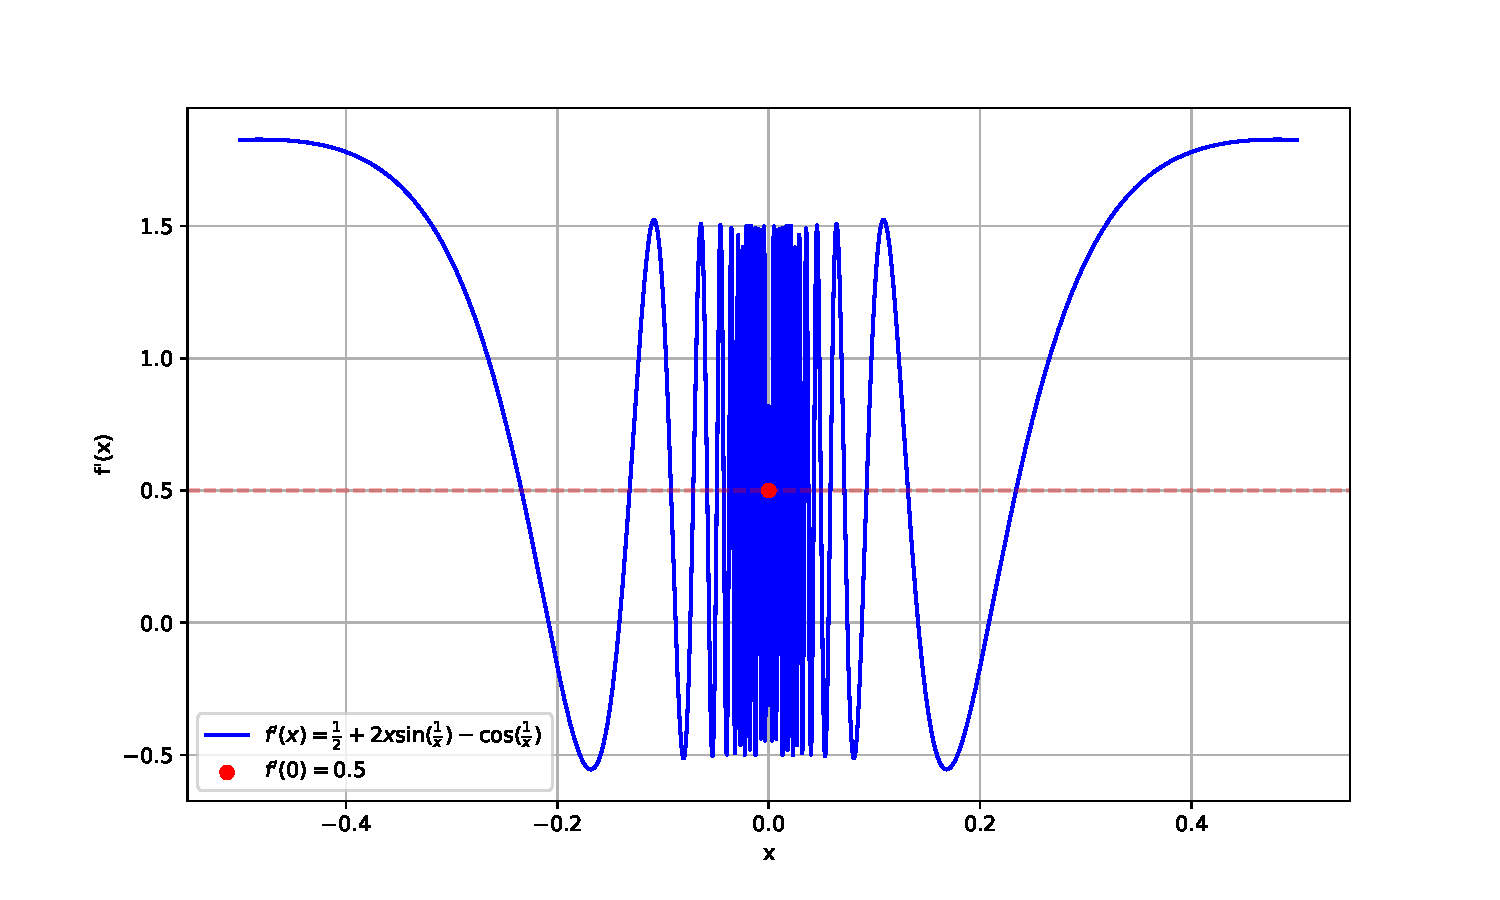
\includegraphics[width=\textwidth]{contraexemplo_crescimento_local.pdf}
    \caption{Gráfico da derivada de $f(x)=\frac{x}{2}+x^2\sin(\frac{1}{x})$}
    \label{fig:contraexemplo_crescimento_local}
\end{figure}

\begin{defn}
    Seja \(f : X \to \R\). Diz-se que \(f\) tem um \emph{máximo local} em \(a \in X\) se existe um \(\delta > 0\) tal que para todo \(x \in X\) com \(|x - a| < \delta\), temos \(f(x) \leq f(a)\). Quando \(x \in X\), \(|x - a| < \delta\) implicam \(f(x) < f(a)\), diz-se que \(f\) tem um \emph{máximo local estrito} em \(a\). Definições são análogas para \emph{mínimo local} e \emph{mínimo local estrito}.
\end{defn}

\begin{defn}
    Seja \(f : X \to \R\). Diz-se que \(f\) tem um \emph{máximo absoluto (global)} em \(a \in X\) se \(f(x) \leq f(a)\) para todo \(x \in X\). Se vale \(f(a) \geq f(x)\) para todo \(x \in X\), diz-se que \(a\) é um \emph{mínimo absoluto (global)} de \(f\).
\end{defn}

\begin{cor}
    Se \(f: X \to \R\) é derivável à direita em \(a \in X \cap X_{+}^{'}\) e tem aí um máximo local então \(f_{+}'(a) \leq 0\).
\end{cor}

\begin{cor} \label{cor:maximos_minimos_derivada_zero}
    Seja \(a \in X\) um ponto de acumulação bilateral. Se \(f : X \to \R\) é derivável no ponto \(a\) e possui aí um máximo ou mínimo local então \(f'(a) = 0\).
\end{cor}

\begin{rem}
    Se \(f: X \to \R\) possui máximo ou mínimo local em \(a \in X\), não se pode concluir que \(f'(a)=0\). Primeiro, \(f'(a)\) pode não existir (e.g., \(f: \R \to \R\), dada por \(f(x)=\vert x \vert\), tem mínimo (global) em \(x=0\) mas não é derivável nesse ponto). Segundo, \(a \in X\) pode não ser ponto de acumulação bilateral (e.g., \(f: [0,1] \to \R\), dada por \(f(x)= x\), possui mínimo (global) em \(x=0\) mas \(f'(0)=1\), pois \(0\) não é ponto de acumulação à esquerda).
\end{rem}

\begin{defn}
    Um ponto \(c \in X\) chama-se \emph{ponto crítico} da função derivável \(f: X \to \R\) quando \(f'(c) = 0\).
\end{defn}

\begin{rem}
    Nem todo ponto crítico é ponto de mínimo ou de máximo local (e.g., \(f: \R \to \R\), dada por \(f(x)=x^3\), admite ponto crítico \(x=0\) mas não tem máximo nem mínimo local).
\end{rem}

\subsection{Funções deriváveis num intervalo}

\begin{thm} [Darboux]
    Seja \(f: [a,b] \to \R\) derivável\footnote{Se \(f'(x)\) é contínua, o resultado segue de \eqref{thm:tvi}}. Se \(f'(a) < d < f'(b)\) então existe \(c \in (a,b)\) tal que \(f'(c) = d\).
\end{thm}

\begin{proof}
    Considere a função auxiliar \(g: [a,b] \to \R\) definida por \(g(x)=f(x)-d\cdot x\). Então \(g'(a)=f'(a)-d<0<f'(b)-d=g'(b)\). De \eqref{prop:crescimento_local}, existem \(\delta_1, \delta_2 > 0\) tais que \(a<x<a+\delta_1 \implies g(a)>g(x)\) e \(b-\delta_2,x,b \implies g(b)>g(x)\). Como \(g\) é contínua no compacto \([a,b]\), o Teorema de Weierstrass \eqref{thm:weierstrass} garante que \(g\) atinge seus pontos de máximo e de mínimo. Seja \(c \in [a,b]\) tal que \(g(c) \leq g(x)\) para todo \(x \in [a,b]\). Vimos que \(c \notin \{a,b\}\), logo \(c \in (a,b)\), donde tem-se \(g'(c) = 0 \iff f'(c) = d\).
\end{proof}

\begin{thm} [Rolle] \label{thm:rolle}
    Seja \(f: [a,b] \to \R\) contínua, com \(f(a)=f(b)\). Se \(f\) é derivável em \((a,b)\) então existe \(c \in (a,b)\) tal que \(f'(c)=0\)
\end{thm}

\begin{proof}
    Pelo Teorema de Weierstrass \eqref{thm:weierstrass}, a função \(f\) contínua no compacto \([a,b]\) atinge seus valores de mínimo e de máximo. Se esses valores ocorrem nas extremidades, de \(f(a)=f(b)\) tem-se que \(f\) é constante, logo \(f'(x)=0\) para todo \(x \in [a,b]\). Caso contrário, um dos pontos de mínimo ou de máximo ocorre num ponto \(c \in (a,b)\), então de \eqref{cor:maximos_minimos_derivada_zero} vem que \(f'(c)=0\).
\end{proof}

\begin{thm} [Teorema do Valor Médio de Lagrange] \label{thm:tvm}
    Seja \(f: [a,b] \to \R\) contínua. Se \(f\) é derivável em \((a,b)\), existe \(c \in (a,b)\) tal que \(f'(c) = [f(b)-f(a)]/(b-a)\).
\end{thm}

\begin{proof}
    O resultado é mera aplicação do Teorema de Rolle \eqref{thm:rolle}. Considera a função auxiliar \(g: [a,b] \to \R\) dada por \(g(x) = f(x) - d\cdot x\). Para se ter \(g(a) = g(b)\), é preciso que \(f(a)-d\cdot a = f(b)-d\cdot b \implies d = [f(b)-f(a)]/(b-a)\). Como \(g\) é contínua em \([a,b]\) e derivável em \((a,b)\) (que seguem das propriedades de funções contínuas e deriváveis), de \eqref{thm:rolle} vem que existe \(c \in (a,b)\) tal que \(g'(c) = f'(c) - d = 0\), donde \(f'(c) = [f(b)-f(a)]/(b-a)\).
\end{proof}

\begin{rem}
    Um enunciado equivalente ao teorema do valor médio de Lagrange é o seguinte: se \(f: [a,a+h] \to \R\) é contínua e derivável em \((a,a+h)\) então existe \(\theta \in (0,1)\) tal que \(f(a+h) = f(a) + h \cdot f'(a + \theta h)\).
\end{rem}

\begin{cor}
    Uma função \(f: I \to \R\), contínua no intervalo \(I\), com derivada \(f'(x)=0\) para todo \(x \in \operatorname{int} I\), é constante.
\end{cor}

\begin{cor}
    Se \(f, g: I \to \R\) são funções contínuas no intervalo \(I\) e deriváveis em \(\operatorname{int} I\), com \(f(x) = g(x)\) para todo \(x \in \operatorname{int} I\) então existe \(c \in \R\) tal que \(g(x) = f(x) + c\) para todo \(x \in I\).
\end{cor}

\begin{cor}
    Seja \(f: I \to \R\) derivável no intervalo \(I\). Se existe \(k \in \R\) tal que \(\vert f'(x) \vert \leq k\) para todo \(x \in I\) então \(x, y \in I \implies \vert f(y)-f(x) \vert \leq k\vert y-x \vert\).
\end{cor}

\begin{rem}
    Se \(f: K \to \R\) é de classe \(C^1\) então \(f\) é \emph{lipschitziana}. De fato, se \(f'\) é contínua num compacto \(K\) então o Teorema de Weierstrass \eqref{thm:weierstrass} garante que \(\vert f'(x) \vert \leq M\) para todo \(x \in K\) e algum \(M > 0\). Tomando o menor intervalo \(I \supseteq K\), vem que \(\vert f(y)-f(x) \vert \leq k\vert y-x \vert\) para todo \(x, y \in I\).
\end{rem}

\begin{cor}
    A fim de que a função derivável \(f: I \to \R\) seja monótona não-decrescente no intervalo \(I\) é necessário e suficiente que \(f'(x) \geq 0\) para todo \(x \in I\).
    Se \(f'(x) > 0\) para todo \(x \in I\) então \(f\) é uma bijeção crescente de \(I\) sobre um intervalo \(J\) e sua inversa \(g: J \to I\) é derivável, com \(g'(y) = 1 / f'(g(y))\) para todo \(y = f(x) \in J\).
\end{cor}

\section{Fórmula de Taylor e Aplicações da Derivada}

\subsection{Fórmula de Taylor}

\begin{defn}
    Denota-se a \(n\)-\emph{ésima derivada} (ou \emph{derivada de ordem \(n\)}) de uma função \(f\) no ponto \(a\) por \(f^{(n)}(a)\). Por definição, \(f^{(n)}(a) \defeq [f^{(n-1)}]'(a)\) para \(n \geq 1\).
    Quando existe \(f^{(n)}(a)\) para todo \(x \in I\), diz-se que a função \(f: I \to \R\) é \(n\) \emph{vezes derivável no intervalo} \(I\). Quando \(f\) é \(n-1\) vezes derivável numa vizinhança de \(a\) e existe \(f^{(n)}(a)\), diz-se que \(f\) é \(n\) \emph{vezes derivável no ponto} \(a\).

    Se \(f\) é \(n\) vezes derivável no intervalo \(I\) e \(f^{(n)}\) é contínua, diz-se que \(f\) é de classe \(C^n\), ou simplesmente \(C^n\). Quando \(f \in C^n\) para todo \(n \in \N\), diz-se que \(f\) é de classe \(C^\infty\). Escrevemos \(f^{(0)} = f\) por convenção, o que quer dizer que \(f\) é uma função contínua.
\end{defn}

\begin{defn}
    Seja \(f: I \to \R\) definida no intervalo \(I\) e \(n\) vezes derivável no ponto \(a \in I\). O \emph{polinômio de Taylor} de ordem \(n\) de \(f\) em torno de \(a\) é o polinômio \(p(h) = a_0 + a_1 h + \cdots + a_n h^n\) cujas derivadas de ordem \(k\) em \(h=0\) coincidem com as derivadas de ordem \(k\) de \(f\) em \(a\), para todo \(k = 0, 1, \ldots, n\). Isto é, \(p^{(k)}(0) = f^{(k)}(a)\) para todo \(k = 0, 1, \ldots, n\). O polinômio de Taylor de ordem \(n\) de \(f\) em torno de \(a\) é então dado por
\begin{equation}
    p(h) = \sum_{k=0}^{n} \frac{f^{(k)}(a)}{k!} h^k.
\end{equation}

    Se \(p(h)\) é o polinômio de Taylor de ordem \(n\) de \(f\) em torno de \(a\), então a função \(r(h) = f(a+h) - p(h)\), definida no intervalo \(J = \{h \in \R : a+h \in I\}\), chamada de \emph{resto} ou \emph{resíduo} da aproximação de \(f\) por \(p\), é \(n\) vezes derivável no ponto \(0 \in J\), com \(r^{(k)}(0) = 0\) para todo \(k = 0, 1, \ldots, n\).
\end{defn}

Antes de provar o Teorema de Taylor, precisamos de um resultado que relaciona o comportamento local de uma função e a velocidade com que ela decai ao nos aproximar desse ponto. O lema a seguir mostra que uma função \(r(h)\) é extremamente achatada no zero (com \(n\) derivadas nulas nesse ponto) sse vai para zero mais rápido que \(h^n\) ao \(h \to 0\).

\begin{lem}
    Seja \(r: J \to \R\) \(n\) vezes derivável no ponto \(0 \in J\). A fim de que seja \(r^{(k)}(0) = 0\) para todo \(k = 0, 1, \ldots, n\) é necessário e suficiente que \(\lim_{h \to 0} r(h)/h^n = 0\).
\end{lem}

\begin{proof}
    Provamos por indução em \(n\). Para \(n=1\), temos \(r(0)=r'(0)=0\) então \(\lim_{h\to 0} r(h)/h = [r(h)-r(0)]/(h-0) = r'(0) = 0\). Supondo que o resultado vale para \(n\), seja \(r\) uma função \(n+1\) vezes derivável em \(0 \in J\), com \(r(0)=r'(0)=\cdots=r^{(n+1)}(0)=0\). Aplicando a hipótese de indução a \(r'(h)\), vem \(\lim_{h\to 0} r'(h)/h=0\). De \eqref{thm:tvm}, existe \(x \in (0,h)\) tal que \(r'(x)h = r(h)\). Então \(\lim_{h \to 0} r(h)/h^{n+1} = \lim_{h \to 0} r'(x)/h^n = \lim_{h \to 0} (r'(x)/x^n) \cdot (x^n/h^n) = 0\) pois \(x \to 0\) ao \(h \to 0\) e \(\vert x/h \vert <1\).
    
    Para provar a volta, usamos indução em \(n\) novamente. No caso de \(n=1\), temos \(\lim_{h\to 0} r(h)/h = 0\) e então \(r(0) = \lim_{h\to 0} h \cdot r(h)/h = 0\) (\(r(0) = \lim_{h \to 0} r(h)\) vem da continuidade de \(r\) em \(0\)) e \(r'(0) = \lim_{h\to 0} [r(h)-r(0)]/(h-0) = 0\). Suponha que o resultado vale para \(n\). Seja \(r\) uma função \(n+1\) vezes derivável em \(0 \in J\) com \(\lim_{h\to 0} r(h)/h^{n+1}=0\) e considere a função \(\varphi: J \to \R\) dada por
    \[
        \varphi(h) = r(h) - \frac{r^{(n+1)}(0)h^{n+1}}{(n+1)!}.
    \]
    Nota que \(\varphi\) é \(n+1\) vezes derivável no ponto \(0\) e \(\lim_{h\to 0} \varphi(h)/h^n = 0\). Pela hipótese de indução, vem que \(\varphi(0) = \varphi'(0) = \cdots = \varphi^{(n)}(0) = 0\), o que implica \(r^{(k)}(0) = 0\) para \(0 \leq k \leq n\). Mas também temos \(\varphi^{(n+1)}(0)= 0\) então (por \(\implies\)) \(\lim_{h\to 0} \varphi(h)/h^{n+1} = 0\). Como \(\lim_{h\to 0} r(h)/h^{n+1} = 0\) por hipótese, concluímos que \(r^{(n+1)}(0)=0\). 
\end{proof}

\begin{thm} [fórmula de Taylor infinitesimal]
    Seja \(f: I \to \R\) \(n\) vezes derivável no ponto \(a \in I\). A função \(r: J \to \R\) dada por \[f(a+h) = \sum_{k=0}^{n} \frac{f^{(k)}(a)}{k!} h^k + r(h),\] no intervalo \(J = \{h \in \R : a+h \in I\}\) obedece \(\lim_{h \to 0} r(h)/h^n = 0\). Reciprocramente, se \(p(h)\) é um polinômio de grau \(\leq n\) tal que \(r(h) = f(a+h) - p(h)\) obedece \(\lim_{h \to 0} r(h)/h^n = 0\) então \(p(h)\) é o polinômio de Taylor de ordem \(n\) de \(f\) no ponto \(a\), isto é, \[p(h) = \sum_{k=0}^{n} \frac{f^{(k)}(a)}{k!} h^k.\]
\end{thm}

\begin{proof}
    
\end{proof}

\begin{thm} [fórmula de Taylor com resto de Lagrange]
    Seja \(f: [a,b] \to \R\) \(n\) vezes derivável no intervalo \((a,b)\), com \(f^{(n-1)}\) contínua em \([a,b]\). Existe \(c \in (a,b)\) tal que \[f(b) = \sum_{k=0}^{n-1} \frac{f^{(k)}(a)}{k!} (b-a)^k + \frac{f^{(n)}(c)}{n!} (b-a)^n.\]
    Colocando \(b=a+h\), vem que \[f(a+h) = \sum_{k=0}^{n-1} \frac{f^{(k)}(a)}{k!} h^k + \frac{f^{(n)}(a+\theta h)}{n!} h^n\] para algum \(\theta \in (0,1)\).
\end{thm}

\begin{proof}
    
\end{proof}

\subsection{Funções convexas e côncavas}

\begin{defn}
    Quando se tem uma função \(f: X \to \R\), definida no conjunto \(X \subseteq \R\), e são dados \(a,b \in X\), o segmento de reta que liga os pontos \((a,f(a))\) e \((b,f(b))\) será chamado a \emph{secante} \(ab\).
\end{defn}

\begin{defn}
    Seja \(I \subseteq \R\) um intervalo. A função \(f: I \to \R\) chama-se \emph{convexa} quando seu gráfico está sempre abaixo de suas secantes, ou seja, para todo \(a<x<b \in I\) tem-se
    \[
        f(x) \leq f(a) + \frac{f(b)-f(a)}{b-a} (x-a),
    \]
    ou também,
    \[
        f(x) \leq f(b) + \frac{f(b)-f(a)}{b-a} (x-b).
    \]
    Juntando as duas desigualdades, tem-se
    \[
        \frac{f(x)-f(a)}{x-a} \leq \frac{f(b)-f(a)}{b-a} \leq \frac{f(b)-f(x)}{b-x}.
    \]
\end{defn}

\begin{prop}
    Se \(f: I \to \R\) é convexa então existem as derivadas laterais \(f_{-}'(c)\) e \(f_{+}'(c)\) para todo \(c \in \operatorname{int} I\).
\end{prop}

\begin{proof}
    
\end{proof}

\begin{cor}
    Uma função convexa \(f: I \to \R\) é contínua em todo ponto interior ao intervalo \(I\).
\end{cor}

\begin{thm} As seguintes afirmações sobre a função \(f: I \to \R\), derivável no intervalo \(I\), são equivalentes:
    \begin{enumerate}
        \item [(1)] \(f\) é convexa;
        \item [(2)] A derivada \(f' : I \to \R\) é monótona não-decrescente;
        \item [(3)] Para todo \(a, x \in I\) tem-se \(f(x) \geq f(a) + f'(a)(x-a)\), ou seja, o gráfico de \(f\) está sempre acima de suas tangentes.
    \end{enumerate}
\end{thm}

\begin{proof}
    
\end{proof}

\begin{cor}
    Todo ponto crítico de uma função convexa é um ponto de mínimo global.
\end{cor}

\begin{cor}
    Uma função \(f: I \to \R\), duas vezes derivável no intervalo \(I\), é convexa sse \(f''(x) \geq 0\) para todo \(x \in I\).
\end{cor}

\begin{defn}
    Uma função \(f: I \to \R\) é \emph{côncava} quando \(-f\) é convexa, ou seja, quando o gráfico de \(f\) está sempre acima de suas secantes.
\end{defn}

\begin{defn}
    Dizemos que uma função \(f: I \to \R\) é \emph{estritamente convexa} (resp. \emph{estritamente côncava}) quando o gráfico de \(f\) está estritamente abaixo (resp. acima) de suas secantes, ou seja, para todo \(a<x<b \in I\) tem-se
    \[
        f(x) < f(a) + \frac{f(b)-f(a)}{b-a} (x-a),
    \]
    no caso convexo, ou com \(>\) em vez de \(<\) no caso côncavo. Segue que o gráfico de \(f\) não possui trechos retilíneos. Conexidade estrita implica que \(f'\) seja crescente mas não implica \(f''(x)>0\) para todo \(x \in I\) (e.g., \(f: \R \to \R\), dada por \(f(x) = x^4\), é estritamente convexa mas \(f''(0)=0\)).
\end{defn}

A desigualdade de Jensen generaliza a afirmação de que o gráfico de uma função convexa está abaixo de suas secantes. Com efeito, se \(f: I \to \R\) é convexa então, dados \(x_1, x_2, \ldots, x_n \in I\) e \(t_1, t_2, \ldots, t_n \in [0,1]\) com \(t_1 + t_2 + \cdots + t_n = 1\), vale
\begin{equation}
    f(t_1 x_1 + t_2 x_2 + \cdots + t_n x_n) \leq t_1 f(x_1) + t_2 f(x_2) + \cdots + t_n f(x_n).
\end{equation}
A prova pode ser feita por indução em \(n\). Usamos este resultado, aplicado à função convexa \(f(x) = e^x\), para mostrar a desigualdade entre a média aritmética e a média geométrica. De fato, com \(t_1 = t_2 = \cdots = t_n = 1/n\) e \(a_1 = \ln x_1, a_2 = \ln x_2, \ldots, a_n = \ln x_n\), vem
\begin{align*}
    \sqrt[n]{x_1 x_2 \cdots x_n} = e^{(a_1 + a_2 + \cdots + a_n)/n} & = e^{t_1 a_1 + t_2 a_2 + \cdots + t_n a_n} \\
    & \leq t_1 e^{a_1} + t_2 e^{a_2} + \cdots + t_n e^{a_n} = \frac{x_1 + x_2 + \cdots + x_n}{n},
\end{align*}
ou seja,
\begin{equation}
    \sqrt[n]{x_1 x_2 \cdots x_n} \leq \frac{x_1 + x_2 + \cdots + x_n}{n}.
\end{equation}

\subsection{Aproximações sucessivas e método de Newton}

\begin{defn}
    Uma função \(f: X \to \R\) chama-se um \emph{contração} quando existe \(k \in [0,1)\) tal que \(\vert f(x)-f(y) \vert \leq k \vert x-y \vert\) para todo \(x, y \in X\).
\end{defn}

\begin{thm} [ponto fixo das contrações]
    Se \(X \subseteq \R\) é fechado então toda contração \(f: X \to X\) tem um único ponto fixo. Mais precisamente, fixando qualquer \(x_0 \in X\), a sequência de aproximações sucessivas \(x_1 = f(x_0)\), \(x_{n+1} = f(x_n)\) converge para o único ponto \(x^* \in X\) tal que \(f(x^*) = x^*\).
\end{thm}

\begin{proof}
    
\end{proof}

Uma aplicação das aproximações sucessivas é o \emph{método de Newton} para encontrar valores aproximados de uma raiz da equação \(f(x)=0\). Neste método, tem-se uma função \(f: I \to \R\) de classe \(C^1\) no intervalo \(I\), com \(f'(x)\neq 0\) para todo \(x \in I\), e um chute inicial \(x_0 \in I\). A sequência de aproximações sucessivas é dada por 
\begin{align}\label{eq:metodo_newton}
    x_1 & = x_0 - f(x_0)/f'(x_0), \\
    x_{n+1} &= x_n - f(x_n)/f'(x_n).
\end{align}
Se a sequência \((x_n)\) converge para um ponto \(x^* \in I\) então \(f(x^*)=0\) pois, fazendo \(n \to \infty\) em \eqref{eq:metodo_newton}, vem \(x^* = x^* - f(x^*)/f'(x^*)\), donde \(f(x^*)=0\). Observa que as raízes de \(f(x)=0\) são exatamente os pontos fixos da função \(g: I \to \R\) dada por
\begin{equation}
    g(x) = x - f(x)/f'(x).
\end{equation}

\begin{prop}
    Se \(f: I \to \R\) é de classe \(C^2\) no intervalo \(I\), com \(f'(x)\neq 0\) para todo \(x \in I\), então cada ponto \(x^* \in \operatorname{int} I\) com \(f(x^*)=0\) tem uma vizinhança \(J = [x^*-\delta, x^*+\delta]\) tal que o método de Newton, com chute inicial \(x_0 \in J\), gera uma sequência de aproximações sucessivas que converge para \(x^*\).
\end{prop}

\begin{proof}
    
\end{proof}

\begin{appendix}

\section{Equivalência assintótica}

\end{appendix}

\end{document}